% put here just enough to compile it 
\documentclass{article}
\usepackage{xcolor}
\usepackage[english]{babel}
\usepackage{graphicx}
\usepackage{docincludes}
\usepackage{siunitx}

\usepackage{hyperref}
\usepackage{cite}
\usepackage{amssymb}
\usepackage{amsmath}
\usepackage{todonotes} % use \todo{WP2Leader: xyz} \todo{ESRz: xyz} or \todo[inline]{} for simple notes.
\usepackage{docincludes} %Added
\usepackage{mathtools} %Added for \prescript
\usepackage{algpseudocode}
\usepackage{algorithm}

\definecolor{deepblack}{rgb}{0,0,0}
\definecolor{deepblue}{rgb}{0,0,0.8}
\definecolor{deepred}{rgb}{0.6,0,0.4}
\definecolor{warningRed}{rgb}{1,0.2,0.2}
\definecolor{deepgreen}{rgb}{0,0.65,0}
\definecolor{commentgreen}{rgb}{0.5,0.7,0.5}






% is the format okay? format?? 
\usepackage[a4paper,top=2cm,bottom=2cm,left=3cm,right=3cm,marginparwidth=1.75cm]{geometry}
\title{Belt drive simulation}

\begin{document}
\begin{titlepage}
\maketitle
\thispagestyle{empty}

\begin{center}
{\includegraphics*[height=3cm]{figures/thread-logo}}
\end{center}

\begin{center}

\includegraphics[scale=0.3]{figures/flag_yellow}
\end{center}
\vspace*{1.3cm}
\begin{center}
\large{\sffamily{This project has received funding from the European Union's Horizon 2020 research and}}\\
\large{\sffamily{innovation programme under the Marie Sk{\l}odowska-Curie grant agreement No 860124.}}
\end{center}

\end{titlepage}
\tableofcontents
%%% Description for the finite element discretisation
%++++++++++++++++++++++++++++++++++++++
%++++++++++++++++++++++++++++++++++++++
% Description of method for exact computation of contact points
\newcommand{\pluseq}{\mathrel{+}=} %for some algorithms ...
%
\section{Methods}
A brief description of cable element, normal and tangential contact model will be added here.
 
%\paragraph{Cable element}
%For the numerical modelling of the belt, a newly developed ANCF beam element was used \cite{Pieber2021}. 
%Note that, however, for the investigations in this test case, the Eulerian axial velocity has been set to zero. A comparison to a model with Eulerian axial velocity set to the overall velocity of the belt drive, see \cite{pechstein2013}, is out of the scope of this test case, but will be performed in future investigations.
%
%
%The geometry of the ANCF beam element with reference length $L$ is defined as follows.
%If $\bar{x} \in [0,L]$ is the local coordinate of the beam element, nodal positions and slopes are given by,
%\be
%\label{eq_Sq}
%  \rv(\bar{x}, t) = \Sm(\bar{x}) \qv(t) \qquad \mbox{and} \qquad 
%  \rv'(\bar{x}, t) = \Sm' (\bar{x}) \qv(t) \eqComma
%\ee
%in which $\qv(t)$ is the vector of generalized coordinates and $\Sm$ is the matrix of shape functions defined as 
%\be
%\Sm(\bar{x})\, =\, \left[\, S_1(\bar{x})\,\Im\;\; S_2(\bar{x})\,\Im\;\; S_3(\bar{x})\,\Im\;\; S_4(\bar{x})\,\Im\, \right] \eqComma
%\ee
%in which $S_i$ are third order polynomials that can be written as,
%\bea
%\label{shapeFunctions}
%  S_1(\bar{x}) &=& 1-3\frac{\bar{x}^2}{L^2}+2\frac{\bar{x}^3}{L^3} \eqComma \quad S_2(\bar{x}) = \bar{x}-2\frac{\bar{x}^2}{L}+\frac{\bar{x}^3}{L^2} \eqComma \nonumber \\
%  S_3(\bar{x}) &=& 3\frac{\bar{x}^2}{L^2}-2\frac{\bar{x}^3}{L^3},\quad S_4(\bar{x}) = -\frac{\bar{x}^2}{L}+\frac{\bar{x}^3}{L^2} \eqComma
%\eea
%
%The description of this subsection follows the implementation of the contact element and can be found in our in-house code Exudyn \cite{2021_Gerstmayr_theDoc}.
%Text, figures and equations in this subsection are widely taken from the documentation \cite{2021_Gerstmayr_theDoc}.
%The description is extended by pseudo-codes as well as specific information that is relevant for the present test case.
%
%\begin{figure}[tbph]
%  \begin{center}
%  \includegraphics[width=12cm]{figures/ESR8_ContactFrictionCircleCable2D.pdf}
%  \end{center}
%      \caption{Sketch of cable, contact segments and circle; showing case without contact, $|\dv_{g1}| > r$, 
%               while contact occurs with $|\dv_{g1}| \le r$; the shortest distance vector $\dv_{g1}$
%               is related to segment $s_1$ (which is perpendicular to the the segment line) and 
%               $\dv_{g2}$ is the shortest distance to the end point of segment $s_2$, not being
%               perpendicular.}
%  \label{fig:ESR8_ObjectContactFrictionCircleCable2D:sketch}
%\end{figure}
%%+++++++++++++++++++++++++++++++++++++++++++++++
%\paragraph{Contact geometry}
%%
%The contact and friction between ANCF cable element and circle is realized with connector elements, each of them per circle and per cable element.
%%
%The connector represents a force element between a circle with radius $R$, which can undergo rigid body motion, and an ANCF cable element as described above.
%%The cable is discretised by splitting into a variable number of segments $s_i$, located between points $p_i$ and $p_{i+1}$. 
%The cable with reference length $L$ is discretised by splitting into $n_{cs}$ straight segments $s_i$, located between points $p_i$ and $p_{i+1}$, compare \fig{fig:ESR8_ObjectContactFrictionCircleCable2D:stickingPos}.
%%
%Note that these points can be placed at a lateral ('vertical') offset from the cable centreline.
%In order to compute the gap function for a line segment, the shortest distance of one line $s_i$ segment (with
%according point vectors $\pv_i$, $\pv_{i+1}$) to the circle centrepoint $\pv_{m0}$ is computed.
%
%With the intermediate quantities (all of them related to segment $s_i$)\footnote{we omit $s_i$ in most terms for brevity!},
%\be
%  \vv_s = \pv_{i+1} - \pv_i, \quad
%  \vv_p = \pv_{m0} - \pv_i, \quad
%  n = \vv_s\tp \vv_p, \quad \mathrm{and} \quad
%  d = \vv_s\tp \vv_s
%\ee
%and assuming that $d \neq 0$,
%%(otherwise the two segment points would be identical and the shortest distance would be $d_g = \Vert \vv_p \Vert $),
%we find the relative position $\rho$ of the shortest (projected) point on the 
%segment, which runs from 0 to 1 if lying on the segment, as
%\be
%  \rho = \frac{n}{d}
%\ee
%We distinguish three cases (see also \fig{fig:ESR8_ObjectContactFrictionCircleCable2D:sketch} for cases 1 and 2):
%    \bn
%    \item If $\rho \le 0$, the shortest distance is the distance to point $\pv_p=\pv_i$,
%    reading 
%    \be
%      d_g = \Vert \pv_{m0} - \pv_i\Vert  \quad (\rho \le 0)
%    \ee
%    \item If $\rho \ge 1$, the shortest distance is the distance to point $\pv_p=\pv_{i+1}$,
%    reading 
%    \be
%      d_g = \Vert \pv_{m0} - \pv_{i+1}\Vert  \quad (\rho \ge 1)
%    \ee
%    \item Finally, if $0 < \rho < 1$, then the shortest distance has a projected point $\pv_p$ somewhere
%    on the segment
%    \be
%      \pv_p = \pv_i + \rho \cdot \vv_s
%    \ee
%    and the distance
%    \be
%      d_g = \Vert \dv_g\Vert  = \sqrt{\vv_p\tp \vv_p - (n^2)/d}
%    \ee
%\en
%Here, the shortest distance vector for every segment results from the projected point $\pv_p$ 
%of the above mentioned cases, see also \fig{fig:ESR8_ObjectContactFrictionCircleCable2D:sketch},
%with the relation
%\be
%  \dv_g = \dv_{g,s_i}= \pv_{m0} - \pv_p \eqDot
%\ee
%The contact gap for a specific point for segment $s_i$ is defined as
%\be \label{ObjectContactFrictionCircleCable2D:gap}
%  g = g_{s_i} = d_g - r \eqDot
%\ee
%using $d_g = \Vert \dv_g\Vert $.
%    
%%++++++++++++++++++++++++++++++++++++++++++++++
%\paragraph{Contact frame and relative motion}
%%FRAME
%The contact normal vector $\nv_{s_i}$ and tangential vector $\tv_{s_i}$ are defined per segment as
%\be
%  \nv_{s_i} = \nv = [n_0, n_1]\tp = \frac{1}{\Vert \dv_{g,s_i}\Vert } \dv_{g,s_i}, \quad \tv_{s_i} = \tv = [-n_1, n_0]\tp
%\ee
%The vectors $\tv_{s_i}$ and $\nv_{s_i}$ define the local (contact) frame for further computations.
%
%The velocity at the closest point of the segment $s_i$ is interpolated using $\rho$ and computed as
%\be
%  \dot \pv_p = (1-\rho) \cdot \vv_i + \rho \cdot \vv_{i+1}
%\ee
%Alternatively, $\dot \pv_p$ could be computed from the cable element by evaluating the velocity at the contact points, but we feel that
%this choice is more consistent with the computations at position level.
%
%The gap velocity $v_n$ ($\neq \dot g$) thus reads
%\be
%  v_n = \left( \dot \pv_p - \dot \pv_{m0} \right) \nv
%\ee
%Similarly, the tangential velocity reads
%\be \label{ObjectContactFrictionCircleCable2D:vTangent}
%  v_t = \left( \dot \pv_p - \dot \pv_{m0} \right) \tv
%\ee
%In order to compute a tangential stiffness, we need a reference point on the circle.
%Thus, we continuously track the sticking position at which the cable element (or segment) and the circle 
%previously sticked together, similar as proposed by Lugr{\'i}s et al.~\cite{lugris2011b}. 
%The difference here to the latter reference, is that we explicitly exclude switching from Newton's method and that Lugr{\'i}s et al.~used
%contact points, while we use linear segments.
%%Furthermore, the bristle model goes back to a regularized version, the so-called LuGre friction model \cite{CanudasDeWitEtAl1993}, by integrating the relative velocity.
%%++++++++++++++++++++++++
%\begin{figure}[tbph]
%  \begin{center}
%  \includegraphics[width=10cm]{figures/ESR8_ContactFrictionCircleCable2DstickingPos.pdf}
%  \end{center}
%  \caption{Calculation of last sticking position; blue parts mark the sticking position calculated as $x^*_{curStick}$.}
%  \label{fig:ESR8_ObjectContactFrictionCircleCable2D:stickingPos}
%\end{figure}
%%++++++++++++++++++++++++
%
%Due to the linear segments, in comparison to the simpler case of contact points, there is the possibility to wind/unwind relative to the (last) sticking position without slipping.
%%
%Therefore, the method to compute the current or last sticking position is more involved.
%In case of sliding, 
%we compute the current sticking position, see \fig{fig:ESR8_ObjectContactFrictionCircleCable2D:stickingPos}, as the sum of the relative position at the segment $s$
%\be
%  x_{s,curStick} = \rho \cdot L_{seg}
%\ee
%in which $\rho \in [0,1]$ denotes the relative position of contact at the segment with reference length $L_{seg}=\frac{L}{n_{cs}}$.
%The relative position at the circle $c$ is
%\be
%  x_{c,curStick} = \alpha \cdot r
%\ee
%We immediately see, that under pure rolling\footnote{neglecting the effects of small penetration, usually much smaller than shown for visibility in \fig{fig:ESR8_ObjectContactFrictionCircleCable2D:stickingPos}.},
%\be
%  x_{s,curStick} + x_{c,curStick}  = \mathrm{const}.
%\ee
%Note that the vertical offset from the cable centreline, as shown in \fig{fig:ESR8_ObjectContactFrictionCircleCable2D:sketch},
%as well as the axial stretch are not considered in the calculation of (un-)winding of the segment.
%While a reduction of segment length reduces this effect because less (un-)winding occurs, a more consistent computation of this effect would require an integration of relative motion as stretch influences the local changes of the relative sticking position.
%For the same reason, the proposed example has a smaller height as compared to the original example \cite{pechstein2013}.
%
%The current sticking position $x_{curStick}$ is computed per segment as
%\be  \label{ObjectContactFrictionCircleCable2D:lastCurStick}
%  x^*_{curStick} = x_{s,curStick} + x_{c,curStick}, \quad
%\ee
%%
%Due to the possibility of switching of $\alpha+\phi$ between $-\pi$ and $\pi$, the result is normalized to
%\be \label{ObjectContactFrictionCircleCable2D:curStick}
%  x_{curStick} = x^*_{curStick} - \mathrm{floor}\left(\frac{x^*_{curStick} }{2 \pi \cdot r} + \frac{1}{2}\right) \cdot 2 \pi \cdot r, \quad
%\ee
%which gives $x_{curStick} \in [-\pi \cdot r,\pi \cdot r]$.
%The function floor() is a standardized version of rounding, available in C and Python programming languages.
%In the so-called PostNewtonStep, see below, the last sticking position is computed, $x_{lastStick} = x_{curStick}$, which is also available at the start of every time step.
%
%%++++++++++++++++++++++++++++++++++++++++++++++
%\paragraph{Contact forces: definition}
%%FORCES
%The normal contact force $f_n$ is zero for gap $g > 0$ and otherwise computed from 
%\be \label{ObjectContactFrictionCircleCable2D:contactForce}
%  f_n = k_c \cdot g + d_c \cdot v_n
%\ee
%Note that the linear spring damper model of \eq{ObjectContactFrictionCircleCable2D:contactForce} does not account for 
%nonlinear effects (increase of contact area in Hertzian contact). However, such models are common in reeving systems \cite{lugris2011b}.
%
%Friction forces are primarily based on relative (tangential) velocity at each segment.
%The linear part of the friction force is based on the relative tangential velocity $v_t$ and the velocity penalty parameter $\mu_v$ and reads
%\be
%  f_t^{(lin)} = \mu_v \cdot v_t \eqComma
%\ee
%The linear part is then used to compute a nonlinear tangential contact force.
%%
%%++++++++++++++++++++++++++++++++++++++++++++++
%\begin{figure}[tbph]
%  \begin{center}
%\pythonstyle\begin{lstlisting}
%function [q0, x0] = ImplicitStep(q, x, tol, tolPNS)
%    #This function is iteratively called at every implicit time step
%
%    #set start of step configuration to solution (q,x) of previous step
%    q_startOfStep = q
%    x_startOfStep = x
%    x0 = x
%
%    #discontinuous iteration starts here:
%    converged_PNS = False
%    while not converged_PNS:
%        q0 = q_startOfStep #reset at every PN step
%        #apply Newton method to implicit step
%        
%        converged_Newton = False
%        while not converged_Newton:
%            f = Residual(q0,x0)
%            
%            if norm(f) <= tol:
%              converged_Newton = True
%              break
%            
%            J = Jacobian(q0,x0)
%            
%            #update q0:
%            q0 = q0-inv(J)*f
%        
%        #update x:
%        [x0, errPNS] = PostNewtonStep(q0, q_startOfStep, x0, x_startOfStep)
%        
%        if errPNS <= tolPNS:
%            converged_PNS = True
%
%    #update state for next iteration
%    return [q0, x0]
%
%\end{lstlisting}
%  \end{center}
%  \caption{Pseudocode for implicit step with continuous (\texttt{q}) and discontinuous (\texttt{x}) solution variables and PostNewtonStep (PNS).
%           Note that the PostNewtonStep requires the current state (\texttt{x0}, \texttt{q0}) as well as the state at the start of the time step
%           in order to compute an appropriate update for the data variables. The tolerances \texttt{tol} resp.\ \texttt{tolPNS} are used as convergence
%           criteria for Newton resp.\ PostNewton }
%	\label{fig_ESR8_NonlinearSolver}
%\end{figure}
%
%
%\paragraph{PostNewtonStep}
%In general, a nonlinear solver, see \fig{fig_ESR8_NonlinearSolver}, is used for the computation of every implicit time step.
%Internally, a Newton method -- which requires continuity of the solution with respect to states (positions and velocities of circle and cable) --
%is applied for the solution of every nonlinear implicit time step.
%Switching may only occur outside of this iteration, which is why we introduce data variables, see below.
%Every step is started with values of the previous time step (or the initial values), while current continuous resp.\ discontinuous variables are updated in the 
%Newton resp.\ discontinuous iteration.
%
%The PostNewtonStep, which is the main update function in the discontinuous iteration, computes 3 values per segment, which are used for computation of contact forces, irrespectively of the current geometry of the contact. 
%The PostNewtonStep is called after every full Newton method and evaluates the current state w.r.t.\ the assumed data variables.
%If the assumptions do not fit, new data variables are computed.
%%This is necessary in order to avoid discontinuities in the equations, while otherwise the Newton iterations would not 
%%(or only slowly) converge.
%
%The data variables per segment are
%\be
%  [x_{gap},\, x_{isSlipStick},\, x_{lastStick}]
%\ee
%Here, $x_{gap}$ contains the gap of the segment ($\le 0$ means contact), $x_{lastStick}$ is described in 
%\eq{ObjectContactFrictionCircleCable2D:curStick}, and 
%$x_{isSlipStick}$ defines the stick or slip case,
%\bi
%  \item $x_{isSlipStick} = -2$: undefined, used for initialization
%  \item $x_{isSlipStick} = 0$: sticking
%  \item $x_{isSlipStick} = \pm 1$: slipping, sign defines slipping direction
%\ei
%    
%The basic algorithm in the PostNewtonStep, with all operations given for any segment $s_i$, can be summarized as follows:
%\bi
%  \item [I.] Evaluate gap per segment $g$ using \eq{ObjectContactFrictionCircleCable2D:gap} and store in data variable: 
%        $x_{gap} = g$
%  \item [II.] If $x_{gap} < 0$ and ($\mu_v \neq 0$ or  $\mu_k \neq 0$):
%  \bi
%    \item[II.1] Compute contact force $f_n$ according to \eq{ObjectContactFrictionCircleCable2D:contactForce}
%    \item[II.2] Compute current sticking position $x_{curStick}$ according to \eq{ObjectContactFrictionCircleCable2D:lastCurStick}
%    \item[II.3] Retrieve \texttt{startOfStep} sticking position in $x^{startOfStep}_{lastStick}$ and compute and normalize
%    difference in sticking position\footnote{in case that $x_{isSlipStick} = -2$, meaning that there is no stored sticking position, we set $\Delta x_{stick} = 0$}:
%    \be
%      \Delta x^*_{stick} = x_{curStick} - x^{startOfStep}_{lastStick}, \quad
%      \Delta x_{stick} = \Delta x^*_{stick} - \mathrm{floor}\left(\frac{\Delta x^*_{stick} }{2 \pi \cdot r} + \frac{1}{2}\right) \cdot 2 \pi \cdot r
%    \ee
%    \item[II.4] Compute linear tangential force for friction stiffness and velocity penalty: 
%      \be 
%        f_{t,lin} = \mu_v \cdot v_t + \mu_k \Delta x_{stick}
%      \ee
%    \item[II.5] Compute tangential force according to Coulomb friction model:
%    \be
%        f_t = 
%            \begin{cases} f_t^{(lin)}, \quad \quad \quad \quad \quad \quad \quad \mathrm{if} \quad 
%              \Vert f_t^{(lin)}\Vert  \le \mu \cdot \Vert f_n\Vert  \\ 
%              \mu \cdot \Vert f_n\Vert  \cdot \mathrm{Sign}(\Delta x_{stick}), \quad \mathrm{else}
%            \end{cases}          
%    \ee
%    \item[II.6] In the case of slipping, given by $\Vert f_t^{(lin)}\Vert  > \mu \cdot \Vert f_n\Vert $, we update the last sticking position in the data variable, 
%    such that the spring is pre-tensioned already,
%    \be
%      x_{lastStick} = x_{curStick} - \mathrm{Sign}(\Delta x_{stick}) \frac{\mu \cdot \Vert f_n\Vert }{\mu_k}, \quad 
%      x_{isSlipStick} = \mathrm{Sign}(\Delta x_{stick})
%    \ee
%    \item[II.7] In the case of sticking, given by $\Vert f_t^{(lin)}\Vert  \le \mu \cdot \Vert f_n\Vert $: Set $x_{isSlipStick} = 0$ and, 
%    if $x^{startOfStep}_{isSlipStick} = -2$ (undefined), we update $x_{lastStick} = x_{curStick}$, while otherwise, $x_{lastStick}$ is unchanged.
%  \ei
%  \item[III.] If $x_{gap} > 0$ or ($\mu_v = 0$ and $\mu_k = 0$), we set $x_{isSlipStick} = -2$ (undefined); this means that in the next step (if this step is accepted), there is no stored sticking position.
%  \item[IV.] Compute an error $\varepsilon_{PNS} = \varepsilon^n_{PNS}+\varepsilon^t_{PNS}$,
%              with physical units forces (per segment point), for \texttt{PostNewtonStep}:
%  \bi
%    \item[IV.1] if gap $x_{gap,lastPNS}$ of previous \texttt{PostNewtonStep} had a different sign as the current gap, set
%    \be
%      \varepsilon^n_{PNS} = k_c \cdot \Vert x_{gap} - x_{gap,lastPNS}\Vert
%    \ee
%    \item[] while otherwise $\varepsilon^n_{PNS}=0$.
%    \item[IV.2] if stick-slip-state $x_{isSlipStick,lastPNS}$ of previous \texttt{PostNewtonStep} is different from current $x_{isSlipStick}$, set
%    \be
%      \varepsilon^t_{PNS} = \Vert \left(\Vert f_t^{(lin)} \Vert  - \mu \cdot \Vert f_n\Vert  \right)\Vert 
%    \ee
%    while otherwise $\varepsilon^t_{PNS}=0$.
%  \ei
%\ei
%
%    \paragraph{Computation of connector forces in Newton}
%    %
%    The computation of the forces produced by the contact-friction element is done during Newton iterations.
%    For efficiency, the force computation is only performed if the \texttt{PostNewtonStep} determined contact in any segment.
%
%    The following operations are performed for each segment $s_i$, if 
%    $x_{gap, s_i} <= 0$:
%    \bi
%      \item[I.] Compute contact force $f_n$, \eq{ObjectContactFrictionCircleCable2D:contactForce}.
%      \item[II.] In case of sticking:
%      \bi
%        \item [II.1] the current sticking position $x_{curStick}$ is computed from \eq{ObjectContactFrictionCircleCable2D:lastCurStick}, and the difference of current and last sticking position reads\footnote{see the difference to the \texttt{PostNewtonStep}: we use $x_{lastStick}$ here, not the \texttt{startOfStep} variant.}:
%        \be
%          \Delta x^*_{stick} = x_{curStick} - x_{lastStick}, \quad
%          \Delta x_{stick} = \Delta x^*_{stick} - \mathrm{floor}\left(\frac{\Delta x^*_{stick} }{2 \pi \cdot r} + \frac{1}{2}\right) \cdot 2 \pi \cdot r
%        \ee
%        \item [II.2] however, if the friction stiffness $\mu_k=0$ or if $x_{isSlipStick} = -2$, we also set $\Delta x_{stick}=0$
%        \item [II.3] using the tangential velocity from \eq{ObjectContactFrictionCircleCable2D:vTangent}, the linear tangent force follows as
%        \be
%          f_{t,lin} = \mu_v \cdot v_t + \mu_k \Delta x_{stick}
%        \ee
%        \item [II.4] the tangential friction force then results in\footnote{see again difference to \texttt{PostNewtonStep}!},
%        \be
%            f_t = 
%                \begin{cases} f_t^{(lin)}, \quad \quad \quad \quad \quad \quad \quad \mathrm{if} \quad 
%                  \Vert x_{isSlipStick} \Vert \neq 1 \\ 
%                  \mu \cdot \Vert f_n\Vert  \cdot x_{isSlipStick}, \quad \mathrm{else}
%                \end{cases}
%        \ee 
%      \ei
%    \ei
%    %++++++++++++++++++++++++++++++++++++++++++++++
%    \paragraph{Computation of generalized forces for circle and ANCF element}
%    Contact forces $\fv_i$ with $i \in [0,n_{cs}]$ are applied at the points $p_i$, and they are computed for every contact segment.
%    For every contact computation, first all contact forces at segment points are set to zero. 
%    In general, we may distinguish two cases, compare \fig{fig:ESR8_ObjectContactFrictionCircleCable2D:normals}.
%    %++++++++++++++++++++++++
%    \begin{figure}[tbph]
%      \begin{center}
%      \includegraphics[width=16cm]{figures/ESR8_ContactFrictionCircleCable2Dnormals.pdf}
%      \end{center}
%      \caption{Choice of normals and tangent vectors for calculation of normal contact forces and tangential (friction) forces; 
%      left: case SN with \texttt{usePointWiseNormals=False};
%      right: case PWN with \texttt{usePointWiseNormals=True} }
%    	\label{fig:ESR8_ObjectContactFrictionCircleCable2D:normals}
%    \end{figure}
%    %++++++++++++++++++++++++
%    Segment normals ($=\,$SN) always lead to good approximations for normal directions, irrespectively of short or extremely long segments as compared to the circle. However, in case of segments that are short as compared to the circle radius, normals computed from the centre of the circle to the segment points ($=\,$PWN) are more consistent and produce tangents only in circumferential direction, which may improve behaviour in some applications. Segment normals are used in the investigations here, reading:
%    \bi
%    \item[] \mybold{CASE SN}: use \mybold{S}egment \mybold{N}ormals\\
%    If there is contact in a segment $s_i$, i.e., gap state $x_{gap} \le 0$, see \fig{fig:ESR8_ObjectContactFrictionCircleCable2D:sketch} (right), contact forces $\fv_{s_i}$ are computed per segment,
%    \be
%      \fv_{s_i} = f_n \cdot \nv_{s_i} + f_t \tv_{s_i}
%    \ee
%    and added to every force $\fv_i$, initialized with zero, at segment points according to
%      \bea
%        \fv_i &=& \fv_i + (1-\rho) \cdot \fv_{s_i}      \\ \nonumber
%        \fv_{i+1} &=& \fv_{i+1}  + \rho \cdot \fv_{s_i}
%      \eea
%    while in case $x_{gap}  > 0$ nothing is added.
%    \ei
%    The forces $\fv_i$ are then applied to the ANCF cable element at according segment points.
%    The forces on the circle (pulley) are computed as the total sum of all
%    segment contact forces, 
%    \be
%      \fv_{m0} = -\sum_{s_i} \fv_{s_i} 
%    \ee
%    and additional torques on the circle's rotation simply follow from
%    \be
%      \tau_{m0} = -\sum_{s_i} r \cdot f_{t_{s_i}} \eqDot
%    \ee
%   
\section{Belt drive simulation}\label{sec:beltdrive}
In this section, we investigate the dynamics of a belt drive system featuring two pulleys, $P_1$ and $P_2$, both with identical radius and inertia, as illustrated in \fig{fig:ESR8_BeltDrive}. The numerical modeling of this system relies on the Absolute Nodal Coordinate Formulation (ANCF), with the pulleys simulated as rigid bodies and the belt-pulley contact modeled as per \cite{Ntarladima2023}.
The repository for the code related to this section is located at:
\bi
  \item[] \url{https://github.com/THREAD-2-3/beltDriveSimulation}
\ei

\subsection{Description of belt drive simulation}
The examined belt drive has two pulleys $P_1$ and $P_2$ with identical radius and inertia, see the geometrical setup in \fig{fig:ESR8_BeltDrive}.
%
The numerical modeling of the belt is based on the Absolute Nodal Coordinate Formulation, \cite{Gerstmayr2008}. The pulleys are simulated as rigid bodies while the contact between the belt and pulleys is modeled as described in \cite{Ntarladima2023}.


%
This numerical example is similar to the one developed in \cite{Pechstein2013} with some modifications which attempt to eliminate the vibrations at the beginning of the simulation and allow the system to reach the steady state. The angular velocity of pulley $P_1$ is prescribed using an algebraic constraint, while some resistance torque over time is added to pulley $P_2$, see the description hereafter.
%++++++++++++++++++++++++++++++++++++++++++++++++++++++++++++++++++++++
\begin{figure}[tbph]
    \centering
    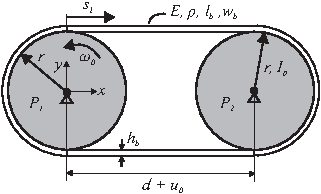
\includegraphics[width=0.55\textwidth]{figures/ESR8_beltPechstein.pdf}
    \caption{Belt drive with two pulleys, displaced from the initial position by $u_0$.}
    \label{fig:ESR8_BeltDrive}
\end{figure}
%++++++++++++++++++++++++++++++++++++++++++++++++++++++++++++++++++++++
\begin{table}[tbph]
    \caption{Main parameters for the belt drive.} \label{tab_beltdriveParameters}
    \centering
    %\begin{tabular}{@{}lrlp{0.4\textwidth}@{}} \toprule
    \begin{tabular}{c|c|c|c|c} \hline
        Par. & Value & Units & Description & variable name in code\\ \hline 
        $r$ & 
            $0.09995$ & \si{\meter} &
            pulley radius & \pythoninline{radiusPulley} \\
        $d$ & 
            $0.1 \pi$ & \si{\meter} &
            distance between two pulleys & \pythoninline{distancePulleys} \\
        $h_b$ & 
            $0.0001$ & \si{\meter} & 
            belt height &\pythoninline{hc} \\
        $w_b$ & 
            $0.08$ & \si{\meter}  & 
            belt width &\pythoninline{b} \\
        $\bar l_b$ & 
            $0.38 \pi$ &  \si{\meter} &  stress-free belt length & (computed)
            \\
        $l_b$ & 
            $0.4 \pi$ &  \si{\meter} &
            initial, deformed belt length & (computed)\\
        $\varepsilon_{ref}$ & 
            $-0.05$ &  - &
            added reference axial strain %of the belt
             & \pythoninline{preStretch}\\% (causing pre-tension)\\
%        $u_0$ & 
%            $0.$ & \si{\meter} &
%            horizontal displacement (used only in original model \cite{Pechstein2013})\\
 %       $E$ & 
%            $10^7$ & \si{\newton \per \meter \squared} &
 %           Young's modulus \\
        $EA$ & 
            $8000$ & \si{\newton \meter} &
            axial stiffness & \pythoninline{EA} \\ 
        $EI$ & 
            $\frac{4}{3} \cdot 10^{-3} $ & \si{\newton \meter \squared} &
            bending stiffness & \pythoninline{EI}\\             
        $\rho$ & 
            $1036$ & \si{\kilogram \per \meter ^3}&
            beam density & \pythoninline{rhoA}\\
        $dEA$ & 
            $1$ & \si{\newton \per {\meter \second}\squared} &
            strain proportional damping & \pythoninline{dEA} \\ 
        $\omega_{P1}$ & 
            $12$ & rad \si{\per \second} & 
            angular velocity of $P_1$ & \pythoninline{omegaFinal}\\
        $d_{P2}$ & 
            $2$ & \si{\newton \meter \per {\second}} &
            %angular velocity proportional 
            damping at $P_2$ & \pythoninline{rotationDampingWheels}\\ 
        $t_0$ & 
            $0.05$ & \si{\second} & 
            driving start time & \pythoninline{tAccStart}  \\
        $t_1$ & 
            $0.60$ & \si{\second} & 
            driving end time & \pythoninline{tAccEnd} \\
        $t_{\tau 0}$ & 
            $1.0$ & \si{\second} & 
            torque $\tau_{P2}$ starts
            %raised at pulley $P_2$  
            &\pythoninline{tTorqueStart} \\
        $t_{\tau 1}$ & 
            $1.5$ & \si{\second} & 
            torque $\tau_{P2}$
            % at pulley $P_2$ 
            reaches nominal value & \pythoninline{tTorqueEnd}\\
        $I_p$ & 
            $0.25$ & \si{\kilo\gram \per \meter \squared} & 
            moment of inertia of  pulleys & \pythoninline{wheelInertia} \\
        %$\mu$ & 
            %$0.5$ & - & 
            %friction coefficient \\
        %$c_c$ & 
            %$4\cdot 10^9$ & \si{\newton \per \meter ^3} & 
            %contact stiffness \\
        $g$ & 9.81 & \si{\meter \per \second \squared} & gravity & \pythoninline{gVec}
 \\ \hline
        %\bottomrule
    \end{tabular}
\end{table}
%++++++++++++++++++++++++++++++++++++++++++++++++++++++++++++++++++++++
%++++++++++++++++++++++++++++++++++++++++++++++++++++++++++++++++++++++
The belt is modeled as a Bernoulli-Euler beam with bending stiffness $EI$, axial stiffness $EA$, rectangular cross-section with height $h_b$ and width $w_b$, as well as stretch proportional damping, density, and further parameters given in \mytab{tab_beltdriveParameters}.
A linearly increasing angular velocity is prescribed to pulley $P_1$ between $t_0$ and $t_1$:
\be \label{eq:ESR8_torqueP2}
  \omega_{P1}(t) = \begin{cases} 0\,\frac{\si{\radian}}{\si{\second}},\quad \quad \quad \quad \quad \quad \quad \quad \quad \quad\,\;\;\mathrm{if} \quad t < t_{0} \\
                  \omega_{P1} \frac{t-t_{0}}{t_{0}-t_{1}}\quad \quad  \quad \quad \quad \quad \quad \quad \quad \;\mathrm{if} \quad t_{0} < t < t_{1} \\ 
                  \omega_{P1} \, \quad \quad \quad \quad \quad \quad \quad \quad \quad \quad \quad \mathrm{else} \, .
                 \end{cases}
\ee
% by varying the angular velocity between $0$ and $\omega_{P1}$. Hereafter, a constant angular velocity $\omega_{P1}$ is prescribed to pulley $P_1$. 


A torque proportional to the angular velocity is applied to the pulley $P_2$ which represents the damping of rotational motion:
\be \label{eq:ESR8_torqueP2b}
  \tau_{P2}(t) = \begin{cases} 0\,\mathrm{Nm}, \quad \quad \quad \quad \quad \quad \quad \quad \quad \quad \quad \quad \,\;\;\mathrm{if} \quad t < 1 \\
                  25\left(0.5-0.5\cdot \cos\left( 2 (t-1) \pi \right) \right)\mathrm{Nm} \quad \mathrm{if} \quad 1 < t < 1.5 \\ 
                  25\,\mathrm{Nm} \quad \quad \quad \quad \quad \quad \quad \quad \quad \quad \quad \quad \,\,\;\mathrm{else} \, .
                 \end{cases}
\ee

As compared to \cite{Pechstein2013}, we use a much smaller belt height $h_b$ to exclude bending effects and a higher pre-tension (due to pre-stretch), while keeping the axial stiffness $EA$ the same. Furthermore, the bending stiffness is lowered by a factor of $50$, which reduces bending effects, as it would lead to significant deviations from an analytical solution otherwise.
The support of pulley $P_1$ is not displaced during the first $0.05\,$s of the simulation, but the pre-stretch $\varepsilon_{ref}$ is applied before running a static computation, which defines a static equilibrium for the dynamic simulation hereafter.
The contact stiffness has been increased by a factor of $40$ and a tangential stiffness (bristle) model has been included to retrieve highly accurate contact behavior. % To investigate steady-state behaviour, the belt drive is first accelerated up to nominal angular velocity $\omega_{P1}$:

% and in the time range $t=[1\,\mathrm{s}, \; 1.5\,\mathrm{s}]$ an additional torque of $25\,$Nm is added to pulley $P_2$, see \eq{eq:ESR8_torqueP2}. 
%At $t=1\,$s an additional torque is added and raised until $t=1.5\,$s to a constant torque of $25\,$Nm by means of the function



\section{Description of code}
For simulating the system we are using the multibody dynamics code Exudyn \cite{Gerstmayr2022}, see the documentation of Exudyn\footnote{https://github.com/jgerstmayr/EXUDYN}.
%
The \exuUrl{https://github.com/THREAD-2-3/beltDriveSimulation/blob/main/src/beltDriveParameterVariation.py}{code} is divided into sections (1, 2,…, 8) and subsections (A, B, …) for easier documenting and processing: %, see section 3 with subsections (A, B, ..., E):
\bi 
\item{In section 1, we import necessary modules.}
\item{Section 2 creates a multibody system, \pythoninline{mbs}.}
\item{Section 3 consists of the Parameter Function. This function will be repeatedly called from Parameter Variation to update the value of the variables for which we perform variations.} 
\bi
\item{
%In subsection 3.A 
We create a class \pythoninline{P} which contains all parameters for which we can perform Parameter variations. First the parameters are given their default values, see \mytab{tab_dafaultValues}. Then we update the values of varying parameters through:
\pythonstyle
\begin{lstlisting}
	for key,value in parameterSet.items():
		setattr(P,key,value)
\end{lstlisting}		
where \pythoninline{setattr()} is a Python function which sets the value of the attribute of an object.}
%
\begin{table}
    \caption{Default values for parameters} \label{tab_dafaultValues}
    \centering
    \begin{tabular}{c|c|c|c|c} \hline
        %\multicolumn{4}{c}{Nominal simulation parameters} \\ \hline 
        Par. & Value & Units & Description & Name in code \\ \hline 
        $t_{end} $ & 
            $2.45$ & \si{\second} &
            evaluation time & \pythoninline{P.tEnd}\\
        $\mu$ & 
            $0.5$ & - &
            dry friction coefficient & \pythoninline{P.dryFriction} \\
        $n_e$ & 
            $240$ & - & 
            number of elements & \pythoninline{P.nANCFnodes}\\
        $dt$ & 
            $5 \cdot 10^{-5}$ & \si{\second}  & 
            time step size & \pythoninline{P.stepSize} \\
        $n_{seg}$ & 4 & - & number of segments &\pythoninline{P.nSegments} \\    
        $k_c$ & 
            $4 \cdot 10^9$ &  \si{\newton \per \meter^3} &  normal contact stiffness & \pythoninline{P.contactStiffnessPerArea *40} 
            \\
        $\mu_k$ & 
            $5 \cdot 10^9$ &  \si{\newton \per \meter^3} &  tangential contact stiffness & \pythoninline{P.frictionStiffnessPerArea}
            \\
        $d_c$ & 
            $8 \cdot 10^4$ &  \si{\newton \second \per \meter^3 }&  normal contact damping & \pythoninline{contactDamping}
            \\
        $\mu_v$ & 
            $ \sqrt{m_{seg} \mu_k} \approx $ &  \si{\newton \second \per \meter^3 } &  tangential contact velocity penalty & \pythoninline{frictionVelocityPenalty}
            \\
            &$3.22\cdot 10^6$ & & &
            \\ \hline
    \end{tabular}
\end{table}
%
\item{
%In subsection 3.B 
We create the model with respect to the parameter values given in  \mytab{tab_beltdriveParameters}}. % which is going to be updated for every parameter variation.}
%
%\item{...}
%
\item{For prescribing the angular velocity, we are using the following user function:
\pythonstyle
\begin{lstlisting}
def UFvelocityDrive(mbs, t, itemNumber, lOffset): 
	if t < tAccStart:  # driving start time
		v = 0
	if t >= tAccStart and t < tAccEnd:
		v = omegaFinal/(tAccEnd-tAccStart)*(t-tAccStart)
	elif t >= tAccEnd:
		v = omegaFinal
	return v
\end{lstlisting}                
}
\begin{table}[hbt!]
    \caption{Input for ObjectANCFCable2D} \label{tab_ObjectANCFCable2D}
    \centering
    %\begin{tabular}{@{}lrlp{0.4\textwidth}@{}} \toprule
    \begin{tabular}{c|c} \hline
        Input & Value \\ \hline 
        \pythoninline{physicsMassPerLength} & $\rho A$\\
        \pythoninline{physicsBendingStiffness} & $EI$\\
        \pythoninline{physicsAxialStiffness} & $EA$\\
        \pythoninline{physicsBendingDamping} & $dEI$\\
        \pythoninline{physicsAxialDamping} & $dEA$\\
        \pythoninline{physicsReferenceAxialStrain}  & $\varepsilon_{ref}$\\
        \pythoninline{physicsReferenceCurvature} & $0$\\
        \pythoninline{useReducedOrderIntegration} & $2$\\
        \pythoninline{strainIsRelativeToReference} & False\\ \hline
        %\bottomrule
    \end{tabular}
\end{table}
\item{For the ANCF beam elements modeling the belt we are using \pythoninline{ObjectANCFCable2D}, see the documentation of Exudyn\footnote{https://github.com/jgerstmayr/EXUDYN}, theDoc.
The input of \pythoninline{ObjectANCFCable2D} is given in \mytab{tab_ObjectANCFCable2D}.}
\item{During the simulation we measure the angular velocity and torque for both pulleys over time,as well as, the axial velocity, the tangential contact stresses, the normal contact stresses and the axial forces over the length of the belt. For this we use \pythoninline{mbs.AddSensor()}. For saving the solution in a different file for each parameter variation we name the solution files using a string which is generated according to the used values for the parameters which can vary:
\pythonstyle
\begin{lstlisting}
    fileClassifier  = ''
    fileClassifier += '-tt'+str(int(P.tEnd*100))
    fileClassifier += '-hh'+str(int(P.stepSize/1e-6))
    fileClassifier += '-nn'+str(int(P.nANCFnodes/60))
    fileClassifier += '-ns'+str(P.nSegments)
    fileClassifier += '-cs'+str(int((P.contactStiffnessPerArea/1e7)))
    fileClassifier += '-fs'+str(int((P.frictionStiffnessPerArea/1e7)))
    fileClassifier += '-df'+str(int(P.dryFriction*10))
    fileClassifier += '-' 
\end{lstlisting} 
For example, for measuring and saving the torque applied to $P_1$ we use:
\pythonstyle
\begin{lstlisting}
 sTorquePulley0 = mbs.AddSensor(SensorObject(objectNumber=velControl, fileName=fileDir+'torquePulley0'+fileClassifier+'.txt',outputVariableType=exu.OutputVariableType.Force))
\end{lstlisting}
}    
\ei
\item{In section 4, simulation settings and visualization settings are defined.}
\item{In section 5, we perform the static and dynamic simulation. %Some parameters such as \pythoninline{frictionCoefficient}, \pythoninline{frictionStiffness} should be given different values during the static simulation. 
We use \pythoninline{mbs.SetObjectParameter} to change objects' parameters after \pythoninline{mbs.Assemble}. This allows us to change the value of some parameters such as \pythoninline{frictionCoefficient}, \pythoninline{frictionStiffness} during the static simulation and to activate or deactivate constrains before and after the static simulation.
For example, before the static simulation we deactivate the constraint which is used for prescribing the angular velocity, \pythoninline{velControl}, by:
\pythonstyle
\begin{lstlisting}
mbs.SetObjectParameter(velControl, 'activeConnector', False)
\end{lstlisting} 
After the static simulation we activate it again.
Note also that we set \pythoninline{updateInitialValues=True} in 
\pythonstyle
\begin{lstlisting}
exu.SolveStatic(mbs, simulationSettings, updateInitialValues=True) 
\end{lstlisting}
which allows us to use the static solution as the initial solution for the dynamic simulation.}
\item{In section 6, the obtained results are post-processed and saved in files.}
\item{In section 7, one can choose between performing single simulation and performing parameter variation.
The option for plotting figures can be chosen as well. All solutions from parameter variations have already been added in \exuUrl{https://github.com/THREAD-2-3/beltDriveSimulation/tree/main/src/solution}{the solution folder}. Solutions from new runs are stored by default in solutionNosync.} %How to use underscore in the text?
\item{In section 8, stored results are plotted. Cases given in \pythoninline{iCases} = $[1,..., 4]$ correspond to different varying quantities; number of elements, step size, other quantities (number of segments, normal contact stiffness, tangential contact stiffness, dry friction coefficient) and evaluation time.}
%

\ei
\section{Installation and running}
\subsection{Installing Python and Exudyn}
The code was tested in a Windows pc using Anaconda, 64bit, Python 3.7.6 and Spyder 4.0.1 which is included in the Anaconda installation.

Exudyn was installed using PIP INSTALLER (pypi.org).
%In order to install Exudyn using pip installer:
Pre-built versions of Exudyn are hosted on \texttt{pypi.org}, see the project
\bi
 \item \exuUrl{https://pypi.org/project/exudyn}{https://pypi.org/project/exudyn}
\ei
For installing Exudyn using pip, as with most other packages, in the regular case (if your binary has been pre-built) you just need to do\footnote{If the index of pypi is not updated, it may help to use \texttt{pip install -i https://pypi.org/project/ exudyn} }
\bi
  \item[] \texttt{pip install exudyn}
\ei
On Linux (currently only pre-built for UBUNTU, but should work on many other linux platforms), {\bf update pip to at least 20.3} and use 
\bi
  \item[] \texttt{pip3 install exudyn}
\ei
For pre-releases (use with care!), add '$--$pre' flag:
\bi
  \item[] \texttt{pip install exudyn $--$pre}
\ei  
  
Results added  
\exuUrl{https://github.com/THREAD-2-3/beltDriveSimulation/tree/main/src/solution}{in src folder}
were obtained using Exudyn V1.2.32.dev1. For installing this version do
\bi
  \item[] \texttt{pip install exudyn==1.2.32.dev1}
\ei
             
For more information for installing Exudyn see the theDoc\footnote{https://github.com/jgerstmayr/EXUDYN}.
%What exactly should I cite here? How to refer to the same footnote?
\subsection{Running the code}
Two python files are added in src folder. One for performing the belt drive simulation with the default values and another for performing variations and plotting figures. (The two files are identical with the only differences being in the flags which are enabling the operations of the code.)
 
For running these files the first option is to open an Anaconda prompt and copy paste the file location.
The second option is to use Spyder and should be selected for making modifications in the code. 

\bibliographystyle{ieeetr}
%\typeout{}
\bibliography{literature}
\end{document}